\documentclass[12pt]{book}
\usepackage{fontspec}
\setmainfont{TeX Gyre Pagella}
\usepackage[paperwidth=8in,paperheight=8in,margin=0.6in]{geometry}
\usepackage{xcolor}
\usepackage{amssymb}
\usepackage{tikz}
\usetikzlibrary{arrows.meta}
\pagestyle{empty}
\setlength{\parindent}{0pt}

\newcommand{\artnote}[1]{{\color{gray!70}\small\itshape [Illustration: #1]}\par\vspace{0.3in}}
\newcommand{\bigline}[1]{{\Huge #1}\par}
\newcommand{\pagenum}[1]{\vfill{\color{gray!50}\footnotesize #1}}
\newcommand{\sprollpage}{\newpage\vspace*{0.4in}}

\begin{document}

\thispagestyle{empty}
\begin{center}
\vspace*{1.1in}
{\Huge \textbf{SPROLL 09}}\\[0.4in]
{\huge \textbf{Parts With a Past}}\\[0.5in]

\begin{tikzpicture}
\draw[line width=1.5pt, gray!50] (0,0) circle (0.4in);
\filldraw[fill=black] (-0.15,0) circle (0.09in);
\filldraw[fill=black] (0.15,0) circle (0.09in);
\end{tikzpicture}
\\[0.4in]
{\large \textit{a whole that still remembers its pieces}}\\[0.3in]
{\small The Sproll Curriculum $\cdot$ Cycle I: Pops}
\end{center}

\sprollpage
\begin{center}
\vspace*{1.5in}
{\Large The Sproll Curriculum}\\[0.2in]
{\normalsize Cycle I --- Pops: Things, Differences, and Counting}\\[0.6in]
{\small Sproll 09 of 40 \quad $\cdot$ \quad follows Sproll 08: When Are They Equal?}
\end{center}
\pagenum{2}

\sprollpage
\begin{center}
\vspace*{0.7in}
\artnote{a single dot from Sproll 00, small in a corner, as a callback}

\begin{tikzpicture}
\filldraw[fill=gray!35] (0,0) circle (0.12in);
\end{tikzpicture}
\vspace{0.35in}
\bigline{Sproll 00 asked:}\vspace{0.1in}
{\Large Can many things be treated as one?}
\end{center}
\pagenum{3}

\sprollpage
\begin{center}
\vspace*{0.6in}
\artnote{two dots sitting near each other, not connected by any line}
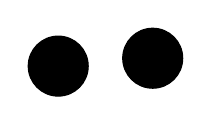
\begin{tikzpicture}
\filldraw[fill=black] (-0.6,0) circle (0.15in);
\filldraw[fill=black] (0.6,0.1) circle (0.15in);
\end{tikzpicture}
\vspace{0.3in}
\bigline{Rule: treat bound things as one.}\vspace{0.1in}
{\Large These are not bound. Still two.}
\end{center}
\pagenum{4}

\sprollpage
\begin{center}
\vspace*{0.7in}
\artnote{the same two dots, now connected by the Bind line from Sproll 05}
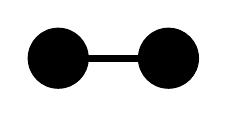
\begin{tikzpicture}
\filldraw[fill=black] (-0.7,0) circle (0.15in);
\filldraw[fill=black] (0.7,0) circle (0.15in);
\draw[line width=2.5pt] (-0.55,0) -- (0.55,0);
\end{tikzpicture}
\vspace{0.35in}
\bigline{Bind them first.}
\end{center}
\pagenum{5}

\sprollpage
\begin{center}
\vspace*{0.7in}
\artnote{the same bound pair, now shown Collapsed under the merging rule into a single larger rounded shape}

\begin{tikzpicture}
\draw[line width=1.5pt, gray!50] (0,0) circle (0.4in);
\filldraw[fill=black] (0,0) circle (0.3in);
\end{tikzpicture}
\vspace{0.35in}
\bigline{Now the rule can call them one.}
\end{center}
\pagenum{6}

\sprollpage
\begin{center}
\vspace*{0.8in}
\artnote{no new image; the unbound pair and the bound-then-merged single shape shown together for comparison}

\begin{tikzpicture}
\filldraw[fill=black] (-1.6,0) circle (0.12in);
\filldraw[fill=black] (-1.0,0.08) circle (0.12in);
\filldraw[fill=black] (1.0,0) circle (0.22in);
\end{tikzpicture}
\vspace{0.35in}
\bigline{Being near each other isn't enough.}\vspace{0.1in}
{\Large Being bound is what the rule needs.}
\end{center}
\pagenum{7}

\sprollpage
\begin{center}
\vspace*{0.5in}
\artnote{three shapes, a dot, a triangle, and a square, all connected to each other by Bind lines}
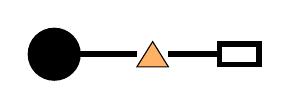
\begin{tikzpicture}
\filldraw[fill=black] (-1.2,0) circle (0.13in);
\draw[fill=orange!60] (-0.15,-0.16) -- (0.05,0.16) -- (0.25,-0.16) -- cycle;
\draw[line width=2pt] (0.9,-0.13) rectangle (1.4,0.13);
\draw[line width=2pt] (-1.05,0) -- (-0.15,0);
\draw[line width=2pt] (0.25,0) -- (0.9,0);
\end{tikzpicture}
\vspace{0.3in}
\bigline{Three bound pieces.}
\end{center}
\pagenum{8}

\sprollpage
\begin{center}
\vspace*{0.7in}
\artnote{the same three pieces, now Collapsed under the merging rule into one larger whole shape}
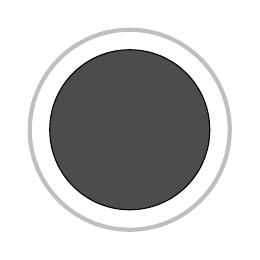
\begin{tikzpicture}
\draw[line width=1.5pt, gray!50] (0,0) circle (0.5in);
\filldraw[fill=black!70] (0,0) circle (0.4in);
\end{tikzpicture}
\vspace{0.35in}
\bigline{One whole.}
\end{center}
\pagenum{9}

\sprollpage
\begin{center}
\vspace*{0.6in}
\artnote{a ledger showing three Pop entries and two Bind entries, the full record behind the whole}
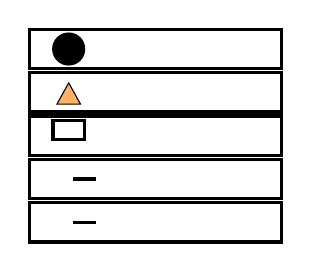
\begin{tikzpicture}
\draw[line width=1.2pt] (-1.6,0.9) rectangle (1.6,1.4);
\filldraw[fill=black] (-1.1,1.15) circle (0.08in);
\draw[line width=1.2pt] (-1.6,0.35) rectangle (1.6,0.85);
\draw[fill=orange!60] (-1.25,0.45) -- (-1.1,0.72) -- (-0.95,0.45) -- cycle;
\draw[line width=1.2pt] (-1.6,-0.2) rectangle (1.6,0.3);
\draw[line width=1.2pt] (-1.3,0) rectangle (-0.9,0.24);
\draw[line width=1.2pt] (-1.6,-0.75) rectangle (1.6,-0.25);
\draw[line width=1.2pt] (-1.05,-0.5) -- (-0.75,-0.5);
\draw[line width=1.2pt] (-1.6,-1.3) rectangle (1.6,-0.8);
\draw[line width=1.2pt] (-1.05,-1.05) -- (-0.75,-1.05);
\end{tikzpicture}
\vspace{0.2in}
\bigline{Ask the history: what made this?}
\end{center}
\pagenum{10}

\sprollpage
\begin{center}
\vspace*{0.7in}
\artnote{the single whole shape from page 9, with a faint, ghostly outline of the three original pieces still visible inside it}
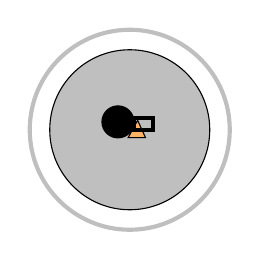
\begin{tikzpicture}
\draw[line width=1.5pt, gray!50] (0,0) circle (0.5in);
\filldraw[fill=black!25] (0,0) circle (0.4in);
\filldraw[fill=black] (-0.15,0.1) circle (0.08in);
\draw[fill=orange!60] (-0.02,-0.1) -- (0.1,0.12) -- (0.2,-0.1) -- cycle;
\draw[line width=1.5pt] (0.05,0) rectangle (0.3,0.15);
\end{tikzpicture}
\vspace{0.3in}
\bigline{The whole does not erase its parts.}\vspace{0.1in}
{\Large The history still remembers them.}
\end{center}
\pagenum{11}

\sprollpage
\begin{center}
\vspace*{0.6in}
\artnote{a simple toy shape (say, a small toy car) built from a few visible interlocking blocks}
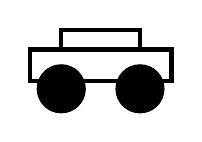
\begin{tikzpicture}
\draw[line width=1.5pt] (-0.9,-0.3) rectangle (0.9,0.1);
\draw[line width=1.5pt] (-0.5,0.1) rectangle (0.5,0.35);
\filldraw[fill=black] (-0.5,-0.4) circle (0.12in);
\filldraw[fill=black] (0.5,-0.4) circle (0.12in);
\end{tikzpicture}
\vspace{0.3in}
\bigline{A toy built from blocks is one toy.}\vspace{0.1in}
{\Large It is still blocks.}
\end{center}
\pagenum{12}

\sprollpage
\begin{center}
\vspace*{0.8in}
\artnote{the whole shape from before, calm and settled, no ghost outline this time}

\begin{tikzpicture}
\draw[line width=1.5pt, gray!50] (0,0) circle (0.4in);
\filldraw[fill=black!70] (0,0) circle (0.32in);
\end{tikzpicture}
\vspace{0.35in}
\bigline{One thing, and many things,}\vspace{0.1in}
{\Large are both true, at the same time.}
\end{center}
\pagenum{13}

\sprollpage
\begin{center}
\vspace*{0.6in}
\artnote{small icons for all four primitives shown together for the first time: a dot for Pop, a crossed-out shape for Refuse, a connecting line for Bind, and a simple lens shape for Collapse}
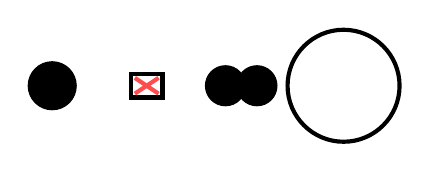
\begin{tikzpicture}
\filldraw[fill=black] (-2.1,0) circle (0.12in);
\draw[line width=1.5pt] (-1.1,-0.15) rectangle (-0.7,0.15);
\draw[line width=1.5pt, red!70] (-1.05,-0.1) -- (-0.75,0.1);
\draw[line width=1.5pt, red!70] (-1.05,0.1) -- (-0.75,-0.1);
\filldraw[fill=black] (0.1,0) circle (0.1in);
\filldraw[fill=black] (0.5,0) circle (0.1in);
\draw[line width=1.5pt] (0.23,0) -- (0.37,0);
\draw[line width=1.5pt] (1.6,0) circle (0.28in);
\end{tikzpicture}
\vspace{0.3in}
\bigline{You now have four moves.}\vspace{0.1in}
{\Large What can you build with all of them together?}
\vspace{0.25in}\\
{\small \textit{--- turn the page for Sproll 10: Four Moves Make a World ---}}
\end{center}
\pagenum{14}

\sprollpage
\vspace*{0.3in}
{\large \textbf{A Note for Grown-Ups}}
\vspace{0.2in}

\normalsize
This book resolves Sproll 00's second open question precisely: many things can be treated as one, but only once they have been Bound and then Collapsed under a rule that specifically merges bound elements. Proximity alone, without Bind, does not qualify, which the unbound-pair page exists to demonstrate directly rather than merely assert.

\vspace{0.15in}
The ghost-outline illustration on page 11 is the book's central image: a Collapse into a whole is not a deletion of the parts, since the underlying history, Pops and Binds, still exists and can still be inspected. This is the beginning of historical mereology, part-whole relations built from events rather than assumed set membership, though this book does not use that term with the child.

\vspace{0.3in}
{\small Sproll 10: Four Moves Make a World continues directly from this book's final page.}
\pagenum{15}

\end{document}
